Có rất nhiều cách để sử dụng EA để khám phá không gian policy trong RL\cite{moriarty1999earl}, trong phần này tôi sẽ mô tả một phương pháp đơn giản để biểu diễn không gian chung policy trong RL. Đó là phương pháp sử dụng một nhiễm sắc thể đơn để biểu diễn một policy với các gen là trọng số của mạng Neural như trong hình \ref{fig:problem:policy}. 
\begin{figure}[ht]
    \centering
    \fbox{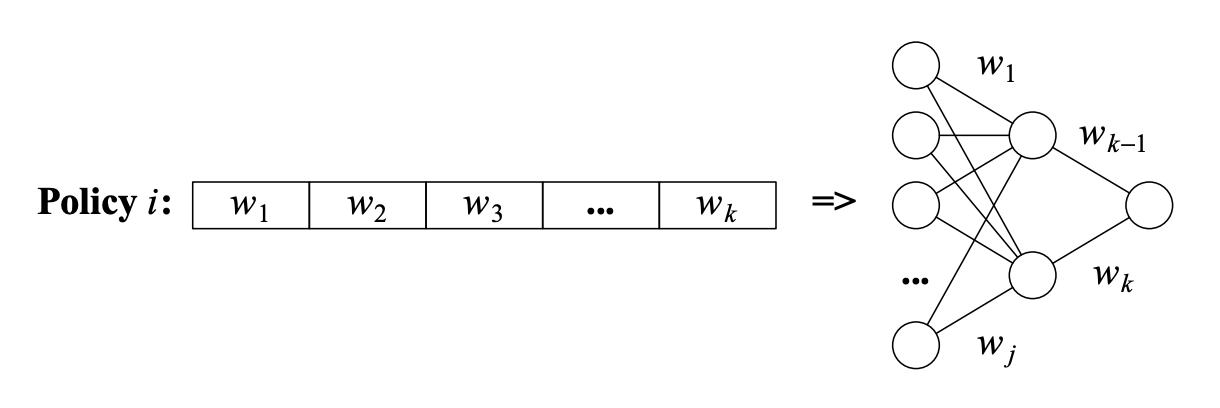
\includegraphics[width=0.7\linewidth]{policy.png}}
    \caption{Cách biểu diễn policy đơn giản bao gồm các trọng số của mạng neural.}
    \label{fig:problem:policy}
\end{figure}
Một mô hình mạng policy được biểu diễn bởi một cấu trúc mạng $H=(h_1,h_2,...h_k)$ có số lớp là $L$ ta sẽ thực hiện tính toán kích thước của không gian chung tương ứng với cấu trúc mạng này:
\begin{align}
    D_{chung} = \sum_{l={1,...L}}(h_{l-1}\cdot h_l + h_l)
\end{align}

Các tham số của mạng sẽ được mã hóa lần lượt vào không gian chung này. Khi cần đánh giá fitness trên một biểu cá thể ta sẽ giải mã từ nhiễm sắc thể về các bộ tham số $w$ và độ lệch $b$ tương ứng để tính tổng phần thưởng thu được với bộ tham số này.

% Quá trình mã hóa và giải mã này được biểu diễn trong hình \ref{fig:problem:policy-decode}.

% Để tìm kiếm tập tham số tối ưu cho \emph{policy}, EA lưu trữ một quần thể với nhiều nhiễm sắc thể khác nhau. Mỗi nhiễm sắc thể trong quần thể có thể được giải mã thành các tham số cho mạng Nơ-ron của \emph{policy}. 

% Tuy nhiên việc giải mã còn phụ thuộc vào ta mã hóa một nhiễm sắc thể như thế nào. Có nhiều phương pháp mã hóa nhiễm sắc thể có thể sử dụng, đa phần chúng được chia thành 2 nhóm:
% \begin{enumerate}
%     \item Mã hóa nhiễm sắc thể gián tiếp nghĩa là chỉ có một số thành phần, cấu trúc bên trong nhiễm sắc thể sẽ tạo lên toàn mạng. 
%     \item Mã hóa nhiễm sắc thể trực tiếp nghĩa là toàn bộ các thành phần, cấu trúc bên trong nhiễm sắc thể sẽ cấu thành lên mạng Nơ-ron.
% \end{enumerate}
